\documentclass[a4paper, twocolumn]{article}
\setlength{\columnsep}{40pt}
\usepackage{graphicx} 
\usepackage[a4paper,margin=0.5in]{geometry}
\usepackage{amsmath}
\usepackage{booktabs}


\title{Hypothesis Testing}
\author{Jawadul Chowdhury}
\date{\today}


\begin{document}

\setlength{\intextsep}{0pt} 
\setlength{\textfloatsep}{5pt} 

\maketitle
\onecolumn
\tableofcontents
\newpage
\twocolumn


\section{Introduction}
In this paper, we explore hypothesis testing by manually creating functions in python for conducting a one sample
t-test, two sample t-test and the pearson's correlation. We explore such methods of hypothesis testing by exploring
a dataset that we will discuss in subsection 1.1.

\subsection{Dataset Description}
For this paper, we work with a dataset from 2009 by the World Health Organization. This dataset tracks a number of 
useful health-related metrics aggregated at the country level. Some features that we will be looking at from the 
dataset is as follows:

\begin{itemize}
    \item Name of the country
    \item Life Expectancy in the Country
    \item Infant Mortality in the country
    \item Physician density
    \item Density of Hospital Beds 
    \item Total Expenditure on Health as Percentage of GDP
    \item Out of Pocket Expenditure as Percentage of Private Expenditure on Health
    \item Per Capita Total Expenditure on Health
    \item Total Fertility Rate 
    \item Gross National Income Per Capita
    \item Name of the Region
\end{itemize}


When we looked at the dataset, we wanted to get more information using \texttt{.info()} and \texttt{.describe()} on
the Pandas data frame we created using the \texttt{.csv} file. Here is the information as follows:

\begin{itemize}
    \item There are a total of 193 rows and 267 columns of data in the dataset
    \item The data types of the features are \texttt{float64}, \texttt{int64} \& \texttt{object}
    \item The dataset in whole takes up a total memory of 402.7+ KB
\end{itemize}

\section{Methods}
In this section, we would like to explore the methods of hypothesis testing that we will be using throughout the
paper, as well as which kind of graphs we will be using for each kind of hypothesis testing and why.

\subsection{One Sample t-test}
A onne sample t-test is meant to compare a numerical variable aginst a fixed number which is specified by us. The
goal is to assess whether the numerical variable is different from the number we've specified. 

To perform the one sample t-test, we need to calculate the test statistic as specified in equation 1.

\begin{equation}
    t = \frac{\mu - M}{\frac{s}{\sqrt{n}}}
    \label{eq:test-statistic}
    \end{equation}
    
    \begin{center}
    Test statistic for one sample
    \end{center}

This is where the standard deviation and $\mu$ is the sample mean, n is the number of observations and M is a 
fixed number is specified by us.

Next, we need to calculate the standard deviation, which is specified in equation 2.

\begin{equation}
    s = \sqrt{\frac{1}{n-1} \sum_{i=1}^{n} (x_i - \mu)^2}
    \label{eq:sample-standard-deviation}
    \end{equation}

    \begin{center}
    Sample standard deviation
    \end{center}

This is where $x_i$ is the value of the variable for the $i^{\text{th}}$ observation. We take the sum of the
differences between $x_i$ and the the $\mu$, and then multiply with 1 over n-1 and then take the square root 
to find the standard deviation. The other variables are similar to the ones explained in equation 1. 

Next, we need to calculate the p-value, which is specified in equation 3.

\begin{equation}
    p = 2(1 - P(|t|))
    \label{eq:p-value}
    \end{equation}
    
    \begin{center}
    P-value
    \end{center}

We calculate the p-value using $P ( \left| t \right|)$ where it is the cumulative distribution function (CDF) for
the t-distribution. 

Lastly, we would like to visualize this. Since we're comparing a numerical variable against a fixed number, it would
be fitting to use a boxplot to help data spread, as this includes the mean, median, lower and upper quartile as well
as any potential outliers. We apply this plotting to the life expectancy of Europe as will be seen in the results
section in Figure 2.

\subsection{Two Sample t-test}
A two-sample t-test is meant to compare a numerical variable against a categorical variable, as the goal is to assess
whether the numerical variable is different across the categories. 

To perform the two sample t-test, we need to calculate the test statistic as specified in equation 4.

\begin{equation}
    t = \frac{\mu_1 - \mu_2}{\sqrt{\frac{s_1^2}{n_1} + \frac{s_2^2}{n_2}}}
    \label{eq:t-test}
\end{equation}
\begin{center}
\text{Test Statistic for two samples}
\end{center}

Here, $\mu_1$, $s_1$ and $n_1$ are the sample mean, sample standard deviation and number of observations from the 
first data set. Next, $\mu_2$, $s_2$ and $n_2$ are the sample mean, sample standard deviation, and number of 
observations from the second second dataset. 

The standard deviation is computed using equation 2 and the p-value is computed using equation 3, with a difference
being the degrees of freedom being used. 

To calculate the degrees of freedom, we need to use equation 5 as specified below, where $\nu$ is the degrees of
freedom.

\begin{equation}
    \nu = \frac{\left(\frac{s_1^2}{n_1} + \frac{s_2^2}{n_2} \right)^2}
{\frac{s_1^4}{n_1^2 (n_1 - 1)} + \frac{s_2^4}{n_2^2 (n_2 - 1)}}
    \label{eq:degree-of-freedom}
\end{equation}
\begin{center}
\text{Degree of Freedom}
\end{center}

Lastly, we would like to visualize this. Since we're comparing a numerical variable against a categorical variable,
it would make the most sense to use a violin plot. In the results section, we will create a violin plot of the life 
expetancy in Europe vs in Asia, as shown in Figure 3 in the Results section.

\subsection{Pearson's Correlation}
The Pearson's Correlation is meant to compare a numerical variale against another numerical variable. We use this to
assess whether the two variables "move" together in a significantly related way. 

To calculate the pearson's correlation, we need to use equation 6 as specified below.

\begin{equation}
    R = \frac{\sum_{i=1}^{n} (x_{i,1} - \mu_1)(x_{i,2} - \mu_2)}
{\sqrt{\sum_{i=1}^{n} (x_{i,1} - \mu_1)^2} \sqrt{\sum_{i=1}^{n} (x_{i,2} - \mu_2)^2}}
    \label{eq:pearson-coefficient}
\end{equation}
\begin{center}
\text{Pearson's Coefficient}
\end{center}

In equation 6 $x_{i,1}$ and $x_{i,2}$ are the $i^{\text{th}}$ observations associated with variable 1 and 2, 
$\mu_1$ and $\mu_2$ are the means of each variable, and n is the number of observations. 

When we do hypothesis testing, we use equation 7 to make the test statistic as specified below.

\begin{equation}
    t = \frac{R \sqrt{n - 2}}{\sqrt{1 - R^2}}
    \label{eq:test-statistic-pearson-coefficient}
\end{equation}
\begin{center}
\text{Test Statistic Pearson's Coefficient}
\end{center}

Once we compute the test statistic, we can then compute the p-value with the degrees of freedom set to $n-2$,
as specified in equation 3.

Lastly, we would like to visualize this. Since we're comparing a numerical variable against another numerical 
variable, it would make the most sense to plot a scatter plot. In the results section, we will create a scatter plot
of the life expectancy vs the infant mortality across the entire dataset, as shown in 4 of the Results section.


\section{Results}
In this section, we explore and analyze the graphs that have been created while performing the different types of
hypothesis testing. 

\subsection{Histogram of Gross National Income}
As shown in Figure 1, we plotted a histogram of the gross national income across all countries in the world that are 
tracked by the World Health Organization. We can observe that the histogram is unimodal and has a right skew. It can
be observed that the mode, median and mean is somewhere between 0 to 10000.

It is also worth noting that there is a peak between 30000 and 40000, however, it might the peak is not high enough
to consider that the histogram is bimodal. 

\begin{figure}[htbp] 
    \centering
    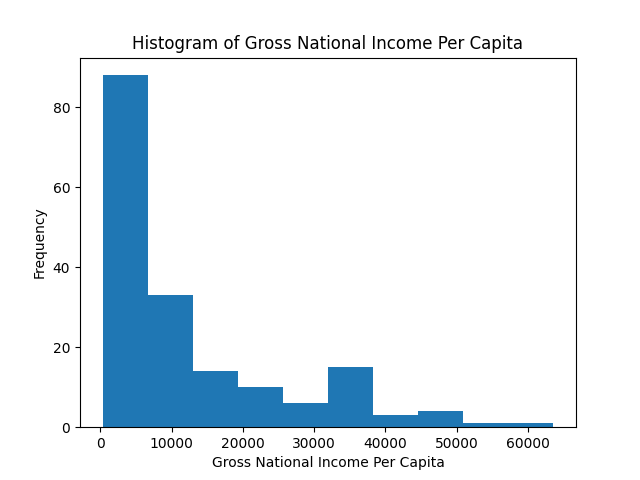
\includegraphics[width=\columnwidth]{C:/GitHub/DataScience/wk_06/plots/GNI_PC.png}
    \caption{Histogram of Gross National Income} 
\end{figure}


\subsection{Boxplot of Life Expectancy in the European Region}
As shown in Figure 2, we plotted a box plot of the life expectancy in the European region. The reason we chose a
box plot is because we're comparing a numerical variable against a fixed number, which is 70 and 76. From this box
plot, we can observe the following summary statistic:

\begin{itemize}
    \item The Lowest Age: 66
    \item The Highest Age: 82
    \item The Lower Quartile: somwhere between 72 and 74
    \item The Upper Quartile: somewhere between 78 and 80
    \item The Median Age: almost around 78
\end{itemize}

\begin{figure}[htbp] 
    \centering
    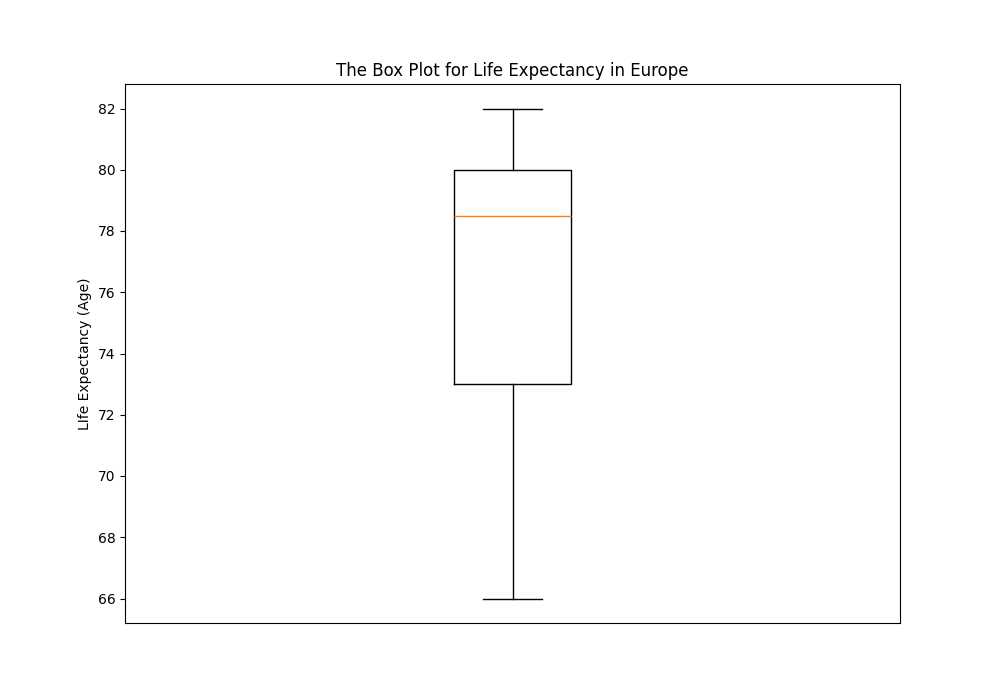
\includegraphics[width=\columnwidth]{C:/GitHub/DataScience/wk_06/plots/BoxPlotLifeExpEU.png}
    \caption{Box Plot of Life Expectancy in Europe} 
\end{figure}


\subsection{Violin Plot of Life Expectancy in Europe \& Asia}
As shown in Figure 3, we plotted a violin plot of the life expectancy in both Europe \& Asia. The reason we chose a 
violin plot is because we're comparing a numerical variable against a categorical variable. From the violin plots,
we can observe a number of things.

\begin{itemize}
    \item It can be seen that around the median, the width of the violin plot is wider, which indicates that there
    are more data points concentrated in that range. 
    \item A striking is difference is that the lowest life expectancy in Europe is somehwere near 60, however, in 
    Asia, it can be as low as between 30 to 40.
    \item The violin plot for Asia has a negative skew, while the violin plot for Europe has a symmetric distribution
    \item It can be seen that Europe has a higher median than Asia, which suggests that the group has a higher
    central value 
\end{itemize}


\begin{figure}[htbp] 
    \centering
    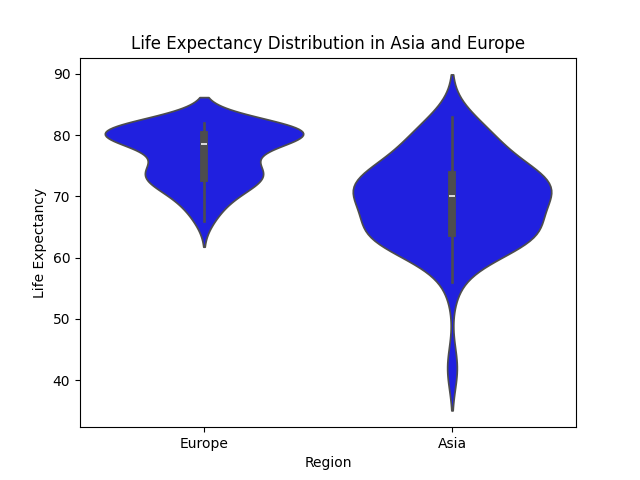
\includegraphics[width=\columnwidth]{C:/GitHub/DataScience/wk_06/plots/ViolinPlotLifeExpEUAS.png}
    \caption{Violin of Life Expectancy in Europe \& Asia} 
\end{figure}

\subsection{Scatterplot of Life Expectancy vs Infant Mortality}
As shown in Figure 4, we plotted a scatter plot of the life expectance vs the infant mortality rate around the world.
The reason we chose a scatter plot is because we're comparing a numerical variable against another numerical 
variable. 

A look at the scatterplot will tell us a number of things:
\begin{itemize}
    \item There is a negative correlation, where as the life expectancy increases, the infant mortality rate decreases
    \item If we were to draw a best fit line, we can see that there is a change in trend from the points being 
    weakly clustered along the line to being strongly clustered as the life expectancy increases
    \item We can deduce that there is a linear relationship between the life expectancy \& infant mortality rate
\end{itemize}

Overall, this suggests that countries that have a high life expectancy means they have low infant mortality rate,
and countries that have a high infant mortality rate have a low life expectancy.

\begin{figure}[htbp] 
    \centering
    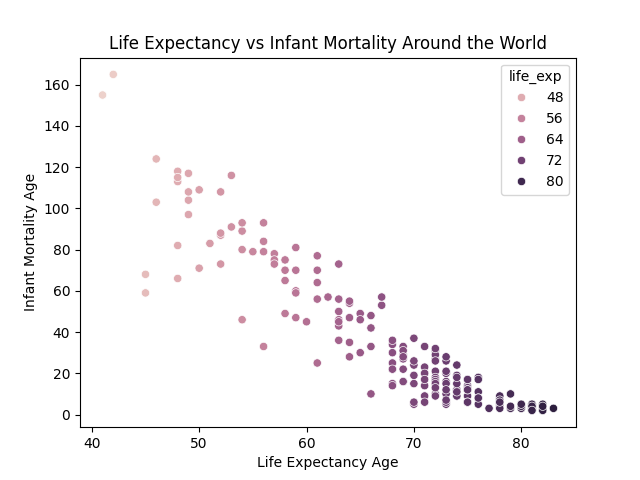
\includegraphics[width=\columnwidth]{C:/GitHub/DataScience/wk_06/plots/ScatterPlot.png}
    \caption{Scatterplot of Life Expectancy vs Infant Mortality} 
\end{figure}


\section{Discussion}
In this last section, we would like to discuss some of the work that has been done in the paper, as well as what
could've been done.

\subsection{The Gross National Income}
In figure 1, we created a histogram of the Gross National Income. As the shape of the distribution is right skewed 
and unimodal, it is worth noting that there was a presence of missing values. We can deal with such missing values
by performing imputations. The imputations can be done using a predictive model such as a KNN, or they can be filled
by calculating the mean, median and mode. A good choice would be to use a KNN model simply because it considers the 
relationships between variables.

\subsection{The One Sample t-test}
For our first hypothesis test, we conducted a one sample t-test. With regards to choosing the M value for our 
experiments, we chose 70 and 76 years because although we didn't know what the life expectancy was, we would like 
to see whether 70 or 76 would be a good estimate for determining what the mean age of the life expectancy is and how 
close we were to being right.

With regards to the value of M, it would make sense to set up a null and alternative hypothesis for the one sample
t-test, which is outlined in the following bullet points:

\begin{itemize}
    \item $H_0$: the mean of the life expectancy in Europe is the same as the value of M
    \item $H_1$: the mean of the life expectancy in Europe isn't the same as the value of M
\end{itemize}




\end{document}